\section{Introduction}

\subsection{What's in the box}

\begin{figure}[H]
\centering
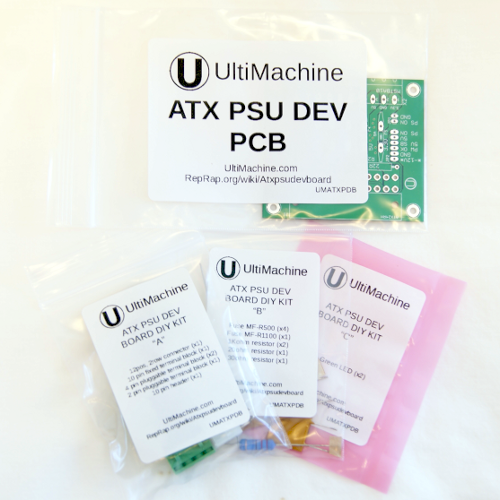
\includegraphics{./png/kit.png}
\caption{Bag Layout}
\end{figure}

\section{Preparation}

\subsection{Tools}

The following tools and materials are required to assemble the ATX PSU
Dev Board:

\begin{itemize}
\itemsep1pt\parskip0pt\parsep0pt
\item
  Soldering Iron
\item
  Solder
\item
  Flush/diagonal cutters
\end{itemize}

Additional tools that might be helpful, but not required:

\begin{itemize}
\itemsep1pt\parskip0pt\parsep0pt
\item
  Lead bender (some 3D printable ones can be found online)
\end{itemize}

\subsection{Soldering}

If you do not have prior experience soldering, we recommend checking out
a few of the following websites for tutorials.

\begin{itemize}
\itemsep1pt\parskip0pt\parsep0pt
\item
  \url{http://mightyohm.com/files/soldercomic/FullSolderComic_EN.pdf}
\item
  \url{http://www.ladyada.net/media/common/soldering.pdf}
\item
  \url{http://store.curiousinventor.com/guides/How_to_Solder}
\item
  \url{http://www.sparkfun.com/tutorials/106}
\item
  \url{http://radiojove.gsfc.nasa.gov/telescope/soldering.htm}
\end{itemize}

\section{Assembly}

\subsection{Board Orientation}

The components of this board will be inserted on the side with the
outlines.

\begin{figure}[H]
\centering
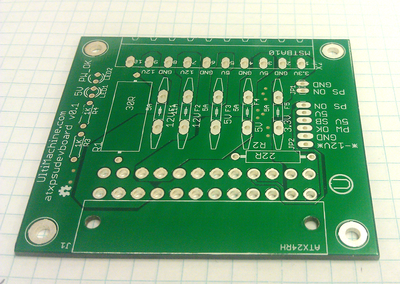
\includegraphics{./png/correct-side.png}
\caption{Correct Side}
\end{figure}

\subsection{Step 1}

Begin by inserting the two 1k ohm
\href{http://en.wikipedia.org/wiki/Resistors}{resistors} and the
\href{http://en.wikipedia.org/wiki/LED}{LEDs} into the board. The LEDs
should have the longest lead in the hole facing the resistor. If they
are inserted incorrectly they will not work. This is because they are
diodes. Diodes only allow current to flow in one direction. Resistors
are not
\href{http://en.wikipedia.org/wiki/Electrical_polarity}{polarized}
components, so they can be inserted in orientation.

\begin{figure}[H]
\centering
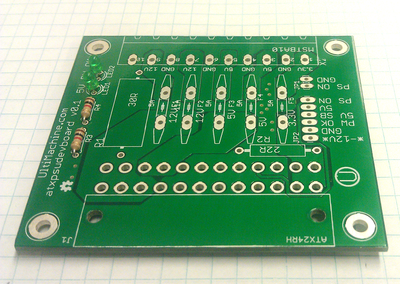
\includegraphics{./png/step-01.png}
\caption{Step 1}
\end{figure}

\subsection{Step 2}

Next flip over the board and solder the components in. You may need to
slightly bend the leads to prevent the componets from falling out of the
board.

\begin{figure}[H]
\centering
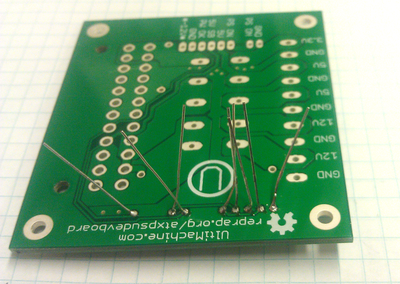
\includegraphics{./png/step-02.png}
\caption{Step 2}
\end{figure}

\subsection{Step 3}

Now that the components are soldered in and secure, you can cut the
leads.

\begin{figure}[H]
\centering
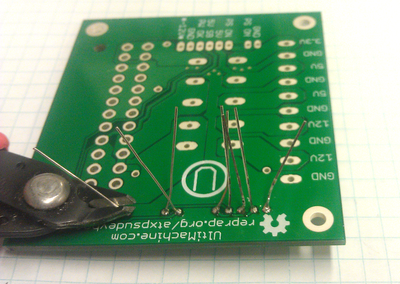
\includegraphics{./png/step-03.png}
\caption{Step 3}
\end{figure}

\subsection{Step 4}

The \href{http://en.wikipedia.org/wiki/Fuse_\%28electrical\%29}{fuses}
will be inserted next. They have a coating that slightly descends down
the leads as shown below.

\begin{figure}[H]
\centering
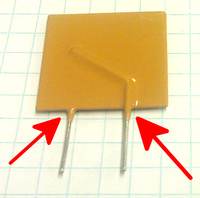
\includegraphics{./png/fuse.png}
\caption{Resetable Fuse}
\end{figure}

In order to make a good connection the fuses should slightly hover over
the holes. This is so the coating on the leads does not interfere with
soldering. You want to bring the fuse above the board. This can be done
with RepRap filament or something else, such as a long screw. The
orientation of the fuses does not matter.

\begin{figure}[H]
\centering
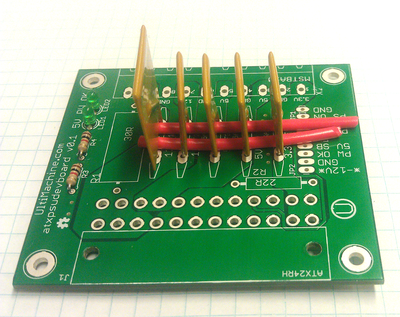
\includegraphics{./png/step-04.png}
\caption{Step 4}
\end{figure}

\subsection{Step 5}

You will need to remove the filament before continuing.

\begin{figure}[H]
\centering
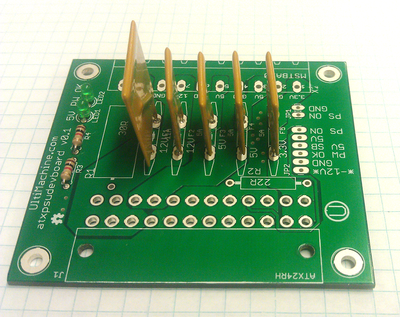
\includegraphics{./png/step-05.png}
\caption{Step 5}
\end{figure}

Now is a good opportunity to inspect the solder joints. Since the
connectors and fuses on this board might carry as much as 10 amps you
want a good solder connection. You can check the quality of the solder
joint by looking at the other side of the leads. A good connection is
shown on the left lead, with a potentially weak one on the right lead.
Add some
\href{http://en.wikipedia.org/wiki/Flux_\%28metallurgy\%29}{flux} and
reheat the joint to touch-up the connections if needed.

\begin{figure}[H]
\centering
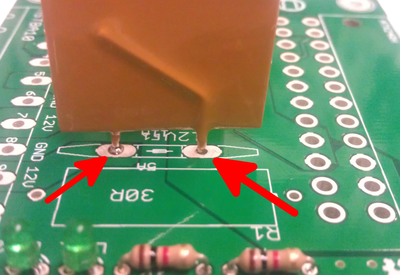
\includegraphics{./png/solder-joint.png}
\caption{Solder Joint}
\end{figure}

\subsection{Step 6}

Next you will want to solder in the remaining resistors. Again,
orientation does not matter for resistors.

\begin{figure}[H]
\centering
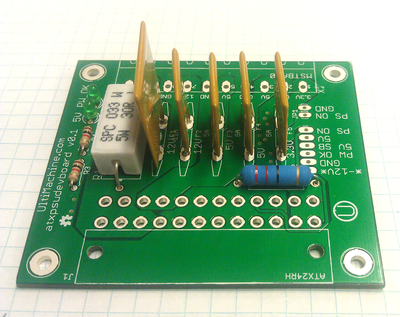
\includegraphics{./png/step-06.png}
\caption{Step 6}
\end{figure}

\subsection{Header Pin Preparation}

Next locate the header pins in the parts bag. You will need to break
them into a strip of 6 and 2 as shown below. This can be done with flush
cutters.

\begin{figure}[H]
\centering
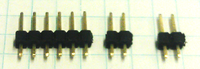
\includegraphics{./png/header-break.png}
\caption{Split header pins}
\end{figure}

\subsection{Step 7}

Solder the header pins as shown.

\begin{figure}[H]
\centering
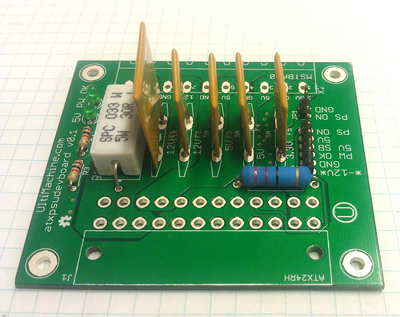
\includegraphics{./png/step-07.png}
\caption{Step 7}
\end{figure}

\subsection{Step 8}

Add the recieving end for the pluggable headers.

\begin{figure}[H]
\centering
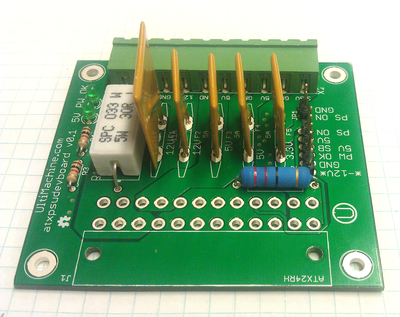
\includegraphics{./png/step-08.png}
\caption{Step 8}
\end{figure}

\subsection{Step 9}

Next you will want to add the ATX connector. It has barbs on the housing
that should clip onto the circuit board. Make sure the connector is well
seated before soldering.

\begin{figure}[H]
\centering
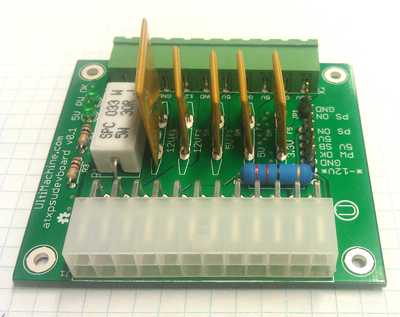
\includegraphics{./png/step-09.png}
\caption{Step 9}
\end{figure}

You have now completed assembly of the ATX PSU Dev Board!

\section{Usage}

In order to turn the power supply on, a jumper between ``PS ON'' and
``GND'' must be added. Optionally, this can be connected to a micro
controller.

\begin{figure}[H]
\centering
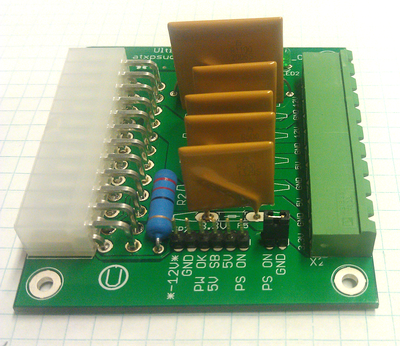
\includegraphics{./png/step-10.png}
\caption{PS\_ON Jumper}
\end{figure}

When an ATX power supply is connected to the board and turned on the
``PW OK'' and ``5V'' light will turn on. Otherwise if not turned on but
connected, just the ``5V'' light will be on.

\begin{figure}[H]
\centering
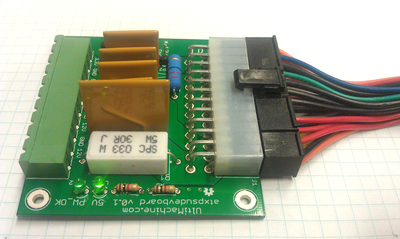
\includegraphics{./png/step-11.png}
\caption{Testing a power supply}
\end{figure}

Finally you can connect the pluggable headers into the board and power
your project!

\begin{figure}[H]
\centering
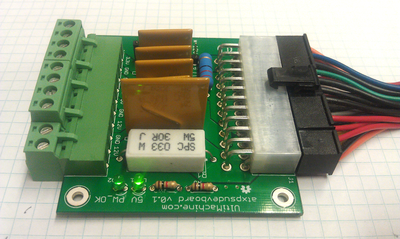
\includegraphics{./png/step-12.png}
\caption{Pluggable headers inserted}
\end{figure}

\section{Source}

The source for the ATX PSU Dev Board can be found in the UltiMachine
repositories on GitHub.com at
\url{https://github.com/ultimachine/ATX-PSU-Dev-Board}.

\section{Issues}

Product support inquiries can be directed to
\href{mailto:info@ultimachine.com}{info@ultimachine.com}. In the event
there is an error in the documentation or problem with the board, please
report the issue to the bug tracker at
\url{https://github.com/ultimachine/ATX-PSU-Dev-Board/issues}.
